\documentclass[titlepage, 11pt]{article}
\usepackage[utf8]{inputenc}
\usepackage[margin=1in]{geometry}
\usepackage{url}
\usepackage{float}
\usepackage{graphicx}
\usepackage{hyperref}
% Define the package name here so we can change it
\newcommand{\pkgname}{\textit{ipprl\_tools}}

\title{\pkgname{} Documentation v1.0}
\date{July 2019}

\begin{document}

\maketitle

\tableofcontents
\section{Compatibility}
The \pkgname{} package was written using Python 3.6, but should be compatible with any version of Python 3 (Python 3.x).

\section{Required Dependencies}
The following packages are required dependencies for the \pkgname{} package. If you installed \pkgname{} through PIP, these dependencies should be installed automatically.

    \begin{itemize}
        \item \textbf{Pandas} $\geq$ v0.23
        \begin{itemize}
            \item \url{https://pandas.pydata.org}
        \end{itemize}
        \item \textbf{NumPy} $\geq$ v1.16
        \begin{itemize}
            \item \url{https://www.numpy.org}
        \end{itemize}
        \item \textbf{SciPy} $\geq$ v1.2
        \begin{itemize}
            \item \url{https://www.scipy.org}
        \end{itemize}
    \end{itemize}

\section{Optional Dependencies}
The following packages are optional dependencies for the \pkgname{} package. These dependencies will not be installed automatically when installing \pkgname{} with PIP, so they must be installed manually if needed.

\begin{itemize}
    \item \textbf{Fuzzy} $\geq$ v1.2.2
    \begin{itemize}
        \item This package is required for the Soundex corruption method. For more information about the package, visit \url{https://pypi.org/project/Fuzzy/}.
    \end{itemize}
    \item \textbf{Jupyter} $\geq$ v1.0.0
    \begin{itemize}
        \item This package is required to view and run the tutorial Jupyter notebook. For more information about Jupyter, visit \url{https://jupyter.org/}
    \end{itemize}
\end{itemize}

\section{Installation}

\subsection{PIP Method (Recommended)}
To install the package via PIP run the command:
\begin{verbatim}
    pip install git+git://github.com/Andrew0Hill/Metrics_Synthetic_Data/
\end{verbatim}
through a command-line interface.
\\
\\
\noindent This command will install the \pkgname{} package into your default Python environment. This command will also install the required dependencies (Pandas, NumPy, SciPy, etc) if they are not already installed. 

\subsection{GitHub Method}: 
The source code can also be cloned directly from GitHub using the following command from a command-line interface.

\begin{verbatim}
    git clone https://github.com/Andrew0Hill/Metrics_Synthetic_Data/
\end{verbatim}

\section{Usage}
\subsection{Importing the Package}
To use \pkgname{}, first import the \verb|synthetic| submodule. 
\begin{figure}[H]
    \centering
    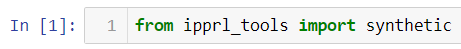
\includegraphics{imgs/Import}
    \caption{Importing \pkgname{}}
    \label{fig:my_label}
\end{figure}

\noindent This command will import all of the functions defined in the \verb|synthetic| submodule. If you only need a subset of the functions, you can specify the exact functions to import as well:

\begin{figure}[H]
    \centering
    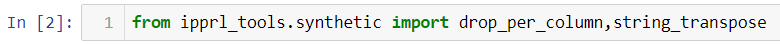
\includegraphics{imgs/Import2}
    \caption{Importing specific functions}
    \label{fig:my_label}
\end{figure}

\subsection{Data Prerequisites}
The synthetic data functions are designed to operate on Pandas DataFrame objects. Pandas DataFrame objects are data structures, similar to R dataframes, which contain data organized in named columns. 
\\
\\
\noindent Before using the synthetic data methods, first read the raw data in as a Pandas DataFrame. The example below shows reading a CSV file in using Pandas.
\\
\noindent For additional ways to import data using Pandas, refer to the Pandas Documentation here:
\\
\href{https://pandas.pydata.org/pandas-docs/stable/user_guide/io.html}{Pandas Documentation: IO}
\\

\begin{figure}[H]
    \centering
    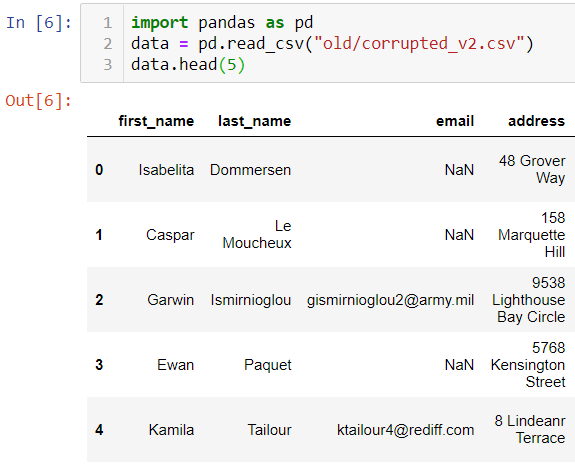
\includegraphics{imgs/PandasRead.png}
    \caption{Reading in a CSV file with Panda}
    \label{fig:my_label}
\end{figure}

\section{Function Documentation}


%% Declaring some documentation macros here

%% Generic macro to make a formatted function description
\newcommand{\parmdesc}[2]{\textit{#1} - #2}

%% Description for the data parameter.
\newcommand{\docdata}{\parmdesc{data}{The Pandas DataFrame to be modified. The DataFrame will be modified in-place.}}

%% Description for the indicators parameter.
\newcommand{\docindc}{\parmdesc{indicators}{A sparse matrix containing information about modified entries in the DataFrame.}}

%% Description for the columns parameter
\newcommand{\doccols}{\parmdesc{columns}{An optional list of columns to operate on. These columns should correspond to column names in the DataFrame being operated on. If this parameter is not passed, defaults to operating on all of the columns in the DataFrame.}}


\subsection{String Manipulation Methods}\label{stringmanip}
String manipulation methods are designed to mimic common typographic errors that can occur when data is entered into a record system.

\subsubsection{\textit{string\_delete(data, indicators, delete\_num, delete\_freq, columns=None)}}

This function randomly deletes characters from strings in one or more columns of the DataFrame. The operation is performed in-place, and information about which values were changed is available in the \textit{indicators} variable.
\\
\\
\textbf{Parameters:}
\begin{itemize}
    \item \docdata
    \item \docindc
    \item \parmdesc{delete\_num}{Parameter choosing an upper bound on the number of deletions per value (i.e. Delete up to 3 characters). This value can either be a scalar \textit{integer} or a list of \textit{integer} to specify a different number of characters for each column to be modified.}
    \item  \parmdesc{delete\_freq}{The percentage of elements in a column which should be modified (i.e. 0.2 == modify 20\% of the values in a column). This value can either be a scalar \textit{float} or a list of \textit{float} to specify a different frequency for each column.}
    \item \doccols
\end{itemize}

 
\subsubsection{\textit{string\_transpose(data, indicators, trans\_num, trans\_freq, columns=None)}}
This function randomly transposes character positions within a string. This operation is intended to simulate a mis-typed entry into a record system.
\\
\\
\textbf{Parameters:}
\begin{itemize}
    \item \docdata
    \item \docindc
    \item \textit{trans\_num} - Parameter specifying an upper bound on the number of transpositions per string value. This value can either be a scalar \textit{integer} or a list of \textit{integer} to specify a different number of characters for each column in \textit{columns}.
    \item \textit{trans\_freq} - The percentage of elements in a column which should be modified (i.e. 0.2 == modify 20\% of the values in the column). This value can also be scalar \textit{float} or a list of \textit{float}.
    \item \doccols
\end{itemize}

\subsubsection{\textit{string\_insert\_alpha(data, indicators, insrt\_num, insrt\_freq, columns=None)}}\label{stinsert}

This function inserts lowercase alphabetical characters (a-z) into a strings randomly. This is to simulate if a field was mistakenly entered with some extraneous characters. 
\\
\\
\textbf{Parameters:}
\begin{itemize}
    \item \docdata
    \item \docindc
    \item \parmdesc{insrt\_num}{Parameter specifying the upper bound on the number of characters to insert into a string. This value can either be a scalar \textit{integer} or a list of \textit{integer} to specify a different upper bound for each column in \textit{columns}}
    \item \parmdesc{insrt\_freq}{The percentage of elements in a column which should be modified. (i.e. 0.2 == modify 20\% of the rows in the column. This can also be a scalar \textit{float} or a list of \textit{float} to specify a different percentage for each column in \textit{columns}. }
\end{itemize}

\subsubsection{\textit{string\_insert\_numeric(data, indicators, insrt\_num, insrt\_freq, columns=None)}}
This function is identical in operation to \textit{string\_insert\_alpha()}, but it randomly inserts numerical characters (0-9) instead of alphabetical characters. This function is suitable for performing corruption on values where alphabetical errors would not be realistic, like in a Phone Number or SSN field.
\\
\\
\textbf{Paramters:}
\\
\textit{See Section \ref{stinsert} for details on parameters.}

\subsection{Replacement Methods}
Unlike the string manipulation methods in Section \ref{stringmanip}, which alter the existing contents of a value by performing string-based manipulations, replacement methods completely change the values contained in a column by replacing each value with another.

\subsubsection{\textit{soundex\_string\_corrupt(data, indicators, corrupt\_name\_pct, columns=None)}}

The Soundex string corruption method works by scanning over the values in each column, and building a Soundex code lookup table that maps Soundex codes to all of the values within the column that contain that Soundex value. 

The function then iterates through each of the values to be replaced, and replaces the original value with another value from the column containing the same Soundex code.

\textbf{Parameters:}
\begin{itemize}
    \item \docdata
    \item \docindc
    \item \parmdesc{corrupt\_name\_pct}{The percentage of values within the column to replace with their Soundex equivalents. This percentage can either be a scalar \textit{float}, or a list of \textit{float} to specify a different percentage for each column in \textit{columns}.}
    \item \doccols
\end{itemize}

\subsubsection{\textit{drop\_per\_column(data, indicators, columns=None, drop\_num = None, drop\_pct=None)}}

The drop-per-column operation randomly chooses some values in the selected columns to delete completely. This operation is intended to simulate missing or incomplete information within a record system. 
\\
\\
A deleted or null value is represented by the empty string "" in the DataFrame. 
\\
\\
\textbf{Parameters:}
\begin{itemize}
    \item \docdata
    \item \docindc
    \item \doccols
    \item \parmdesc{drop\_num}{An optional parameter specifying the number of values to drop as an absolute number of rows. This value may either be a \textit{integer} number of rows, or a list of \textit{integer}  corrseponding to the columns in \textit{columns}. Either this parameter or \textit{drop\_pct} should be specified when calling the function, but not both.}
    \item \parmdesc{drop\_pct}{An optional parameter specifying the number of values to drop as a percentage of the total number of rows. This value may either be a \textit{float} or a list of \textit{float}. Either this value or \textit{drop\_num} should be specified, but not both.}
\end{itemize}

\subsubsection{\textit{edit\_values(data, swap\_set, indicators, pct\_edits, columns=None)}}
This function swaps randomly chosen rows from \textit{data} with randomly chosen rows (from the same column name) from \textit{swap\_set}. 
\\
\\
This function is intended to replicate natural information change over time.
\\
\\
\textbf{Parameters:}
\begin{itemize}
    \item \docdata
    \item \parmdesc{swap\_set}{This parameter should be a Pandas DataFrame with column names that match the column names in \textit{data}. This DataFrame represents the "set" from which values will be randomly chosen to replace values in \textit{data}. }
    \item \docindc
    \item \parmdesc{pct\_edits}{This parameter represents the percentage of values within a column with should be edited. This can either be a scalar \textit{float} or a list of \textit{float} to specify a different percentage for each element of \textit{columns}.}
    \item \doccols
\end{itemize}

\section{Utilities}
In addition to the synthetic data corruption methods, \pkgname{} also provides some utility functions to make generating synthetic datasets easier.
\subsection{Data Utilities}
\subsubsection{\textit{split\_dataset(raw\_data, overlap\_pct)}}
This function is a simple utility that takes a DataFrame as input, then returns two DataFrames containing two separate Datasets, where \textit{overlap\_pct} of the rows from the dataset occur in both DataFrames, and the rests of the rows are unique to their repsective DataFrame.
\\
This function also returns a \textit{ground\_truth} variable, which is a list of tuples containing the IDs of the matching rows in the \textit{left} and \textit{right} datasets.
\\
\textbf{Parameters:}
\begin{itemize}
    \item \parmdesc{raw\_data}{The DataFrame containing the raw data to build the dataset from.}
    \item \parmdesc{overlap\_pct}{The percentage of rows in \textit{raw\_data} which should be used as ground-truth positive linkages. (i.e. 0.5 == 50\% of the rows will be considered as positive linkages in the ground-truth data.}
\end{itemize}
\textbf{Returns:}
\begin{itemize}
    \item \parmdesc{left}{One half of the generated synthetic dataset.}
    \item \parmdesc{right}{The other half of the generated synthetic dataset.}
    \item \parmdesc{ground\_truth}{A list of tuples containing the IDs of the row pairs that overlap between \textit{left} and \textit{right}}
\end{itemize}
\end{document}
